
%\documentclass[12pt]{amsart}
%\usepackage{geometry} % see geometry.pdf on how to lay out the page. There's lots.
%\usepackage{datetime}
%\geometry{a4paper} % or letter or a5paper or ... etc
%% \geometry{landscape} % rotated page geometry
%
%% See the ``Article customise'' template for come common customisations
%
%\title{Wind chapter}
%\author{Percy Link}
%\date{\currenttime \ \today} % delete this line to display the current date
%
%%%% BEGIN DOCUMENT
%\begin{document}
%
%\maketitle

\section{Introduction}

In this chapter, we investigate the effect of changes in land surface heat fluxes, mediated by modifications in soil moisture, on near-surface winds in California.  Understanding and accurate simulation of near-surface winds are necessary for a range of applications, including water vapor and pollutant transport studies, weather forecasting, aviation, and wind energy forecasting.  Here, we focus on wind forecasting for wind energy applications and on winds at a specific wind farm, the Solano Wind Project in the Sacramento-San Joaquin River Delta region of California (38.166N, 121.817W; Figure \ref{fig:windSol_solanomap}).  A regional atmospheric model is used to test the sensitivity of Solano winds to different regions' soil moisture and to quantify the magnitude of the effect at different times of day across a range of soil moisture changes.  We demonstrate that accurate soil moisture information can improve wind forecasts.  This study serves as a prototype for characterizing the importance of soil moisture information for wind forecasts at other wind farms.

\begin{figure}[here]
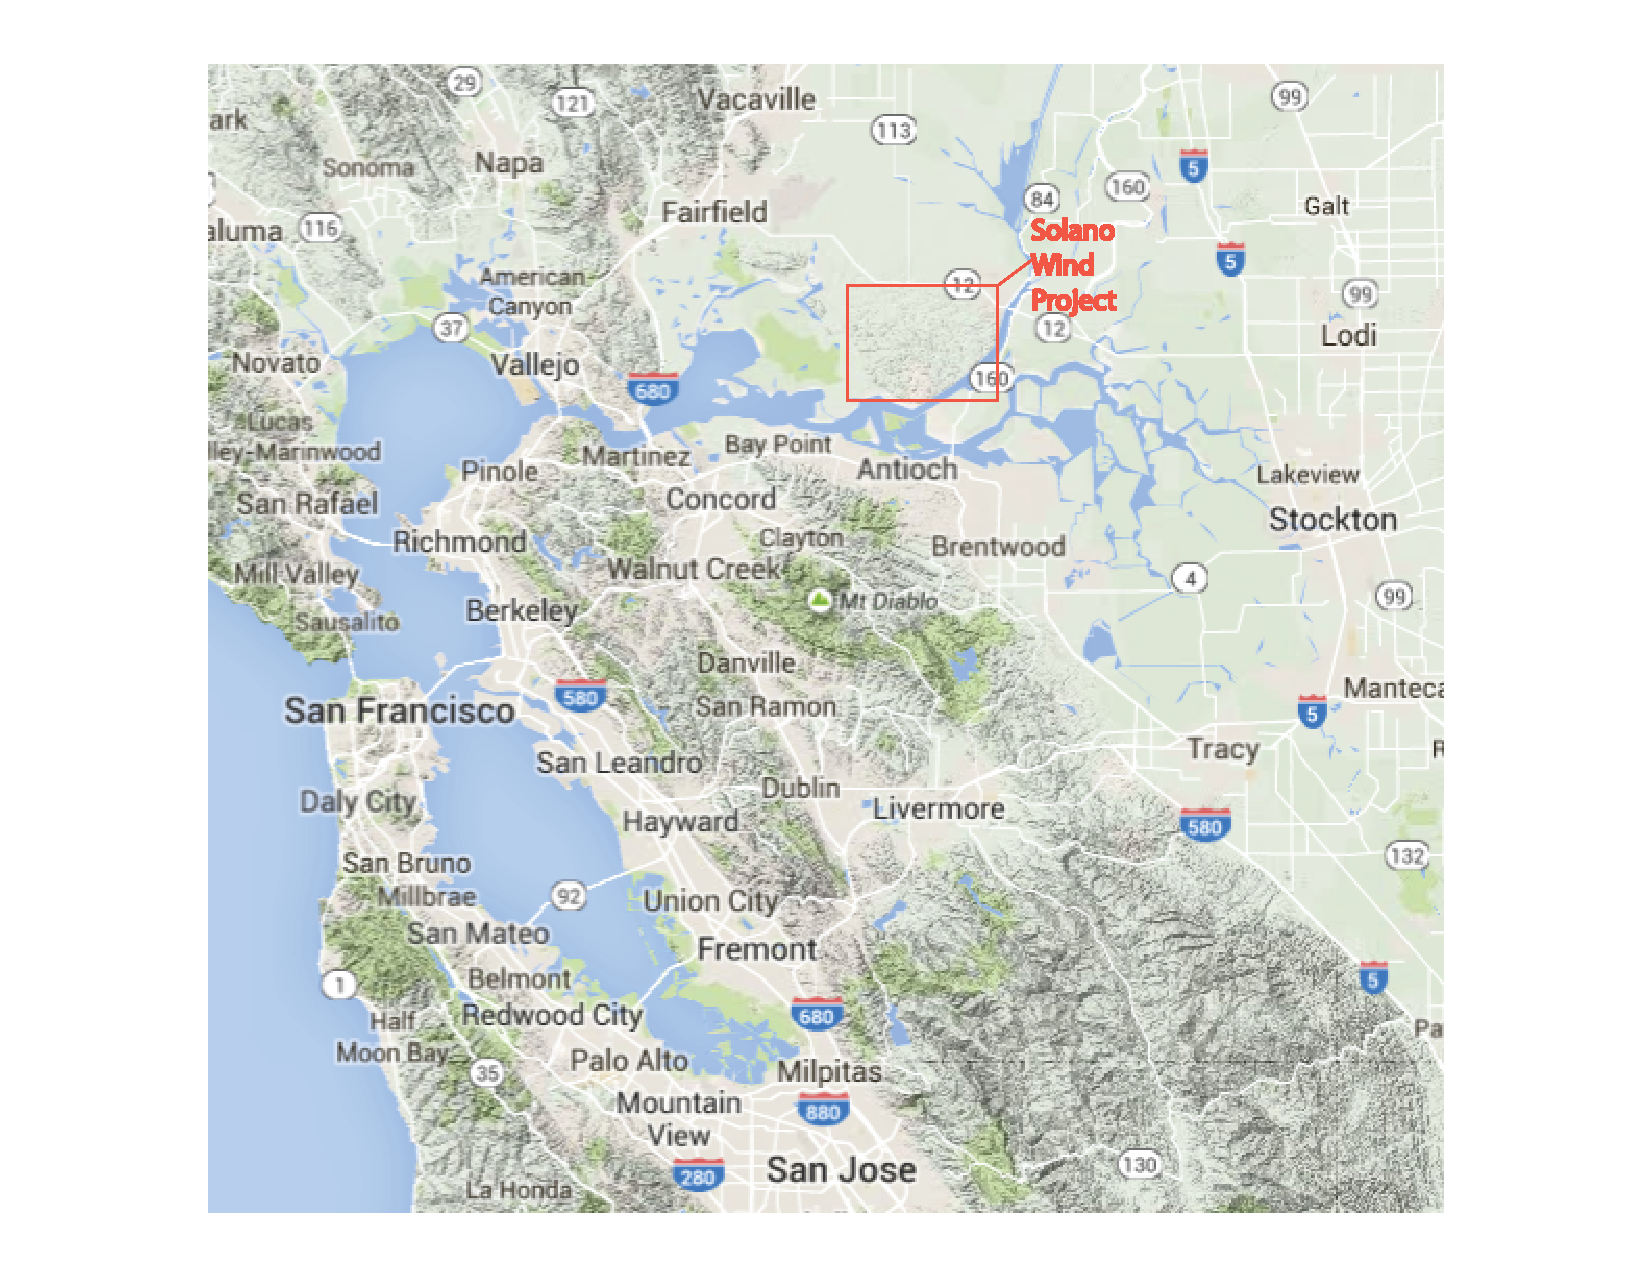
\includegraphics[width=1\textwidth]{ch3-wind/img/solano_map.pdf}
\caption{Location of the Solano Wind Project, in red rectangle.  Credit Google Maps.}
\label{fig:windSol_solanomap}
\end{figure}

Accurate wind forecasts can reduce the cost of integrating wind energy into the electric grid on a large scale.  In order to reduce CO$_2$ emissions to the degree necessary to avert dangerous climate change [\cite{stocker2013ipcc}], electric utilities will need to transition to non-fossil-fuel energy sources, including a large fraction of wind energy [\cite{jacobson2011providing}].  However, even though wind energy has large peak generation potential, it is intermittent, and the instantaneous mismatch between wind generation and electric demand must be met with other power sources.  In most utilities, allocations of conventional electric generation (coal, natural gas, hydroelectric, and nuclear) are made one day in advance, based on forecasted net demand (demand minus wind and solar supply).  At shorter lead times (hour-ahead to real-time), imbalances between the day-ahead allocations of conventional generation and the actual net demand must be met with, in the case of a shortfall, more expensive quick-startup generation, or in the case of excess generation, wasted energy resources.  These imbalance costs add significantly to the cost of wind energy (around 10\% of a wind generator's income in a liberalized market [\cite{fabbri2005assessment}]).  Improved accuracy of wind forecasts could reduce imbalance costs, making integration of wind into the electric grid more economically feasible: wind and solar forecasting could reduce energy costs by \$0.01 to \$0.02 per kWh at 30\% wind and solar penetration [\cite{energy2010western}], or 8-15\% of the average US cost of electricity (\$0.13/kWh in July 2014 [\cite{eia2014}]).

%; and at high wind penetration, \$68 million to \$160 million could be saved annually in California using current state of the art forecasting, with an opportunity to save \$19 million to \$38 million more with forecast accuracy improvements [Porter and Rogers, 2010].

The major wind forecasting companies in North America and Europe use numerical weather prediction (NWP) models to make their day-ahead forecasts, often in combination with statistical post-processing [\cite{porter2010status}; \cite{foley2012current}; \cite{monteiro2009wind}].  NWP models simulate atmospheric wind speed, temperature, pressure, and humidity (among other variables) by solving the equations for conservation of momentum, mass, and energy, discretized in three spatial dimensions and in time.  NWP models require bottom boundary fluxes of energy, moisture, and momentum, but little attention has been paid to these bottom boundary fluxes in the wind energy literature (with the notable exceptions of \cite{marjanovic2014} and \cite{wharton2011review}, discussed below).  Wind energy forecast research has concentrated instead on sensitivity to NWP physical parameterizations, especially planetary boundary layer (PBL) schemes [\cite{draxl2014evaluating}; \cite{marjanovic2014}], and to grid resolution [\cite{marjanovic2014}, \cite{carvalho2012sensitivity}].  There have also been extensive efforts to enhance NWP wind energy forecasts by running model ensembles [\cite{deppe2013wrf}; \cite{pinson2009ensemble}] and by applying various model output statistics (MOS) algorithms [\cite{bedard2013development}; \cite{ranaboldo2013implementation}; \cite{ellis2014predicting}; \cite{ortiz2011short}; \cite{kusiak2009wind}].

%The prediction of ramps (rapid increases or decreases in wind power) remains a challenge [Carcangiu \textit{et al.}, 2014; Ellis \textit{et al.}, 2014; Wharton \textit{et al.}, 2011].

%Regional NWP models require boundary condition information at the lateral boundaries of the grid, as well as bottom boundary fluxes of energy, moisture, and momentum.  If the bottom boundary is land, these fluxes are usually calculated with a land surface model.  

%Wind energy forecasts are sensitive to NWP model resolution and physical parameterizations, especially planetary boundary layer (PBL) schemes [Draxl \textit{et al.}, 2014; Marjanovic \textit{et al.}, 2014]; the optimal PBL scheme depends in part on atmospheric stability conditions [Draxl \textit{et al.}, 2014; Marjanovic \textit{et al.}, 2014], and the optimal grid resolution depends largely on terrain complexity, with more complex terrain requiring higher resolution [Marjanovic \textit{et al.}, 2014, Carvalho \textit{et al.}, 2012].  Ensembles of NWP runs have been used to characterize a forecast probability distribution [Deppe \textit{et al.}, 2013; Pinson and Madsen, 2009].  Various model output statistics (MOS) algorithms incorporating historical observations have been shown to improve NWP forecasts in post-processing; in particular, machine learning algorithms such as directional multipoint linear regression [B\'edard \textit{et al.}, 2013], multiple linear regression [Ranaboldo \textit{et al.}, 2013], random forests, generalized linear models, gradient boosting, and support vector machines [Ellis \textit{et al.}, 2014; Ortiz-Garc\'ia \textit{et al.}, 2011], and neural networks [Kusiak \textit{et al.}, 2009] have shown promise.  The prediction of ramps (rapid increases or decreases in wind power) remains a challenge [Carcangiu \textit{et al.}, 2014; Ellis \textit{et al.}, 2014; Wharton \textit{et al.}, 2011].

The influence of soil moisture and land surface heating on wind prediction has received little attention in the wind energy forecasting literature, even though fluxes of energy at the land surface are known to influence regional circulations.  Soil moisture heterogeneity, and the resulting contrasts in sensible heat flux, can drive mesoscale circulations on land with wind speeds of several m/s [\cite{chen1994impact}; \cite{avissar1998evaluation}].  Thermal contrast between land and ocean can drive sea-breeze circulations with wind speeds up to 10 m/s [\cite{miller2003sea}], and the strength of the thermal contrast and of the resulting wind depends in part on soil moisture because of its influence on land surface temperature [\cite{physick1980numerical}].  In one of the few wind energy papers to discuss the effect of soil moisture on wind forecasts, \cite{marjanovic2014} show that the forecast at a West Coast wind farm is sensitive to initial soil moisture, and in a related study, \cite{wharton2011review} show that soil moisture can be important for forecasting wind ramps, which remain a challenge in wind energy forecasting [\cite{carcangiu2013wind}; \cite{ellis2014predicting}].

California low-level winds are strongly influenced by the contrast of land surface heating with the adjacent cool ocean [\cite{zhong2004diurnal}], and as such, winds at the Solano wind farm are likely to depend on soil moisture.  Solano sits in a wide gap in the Coast Range between the ocean and California's Central Valley (Figure \ref{fig:windSol_domainmap}, red star), and onshore winds are channeled and accelerated through the gap; this topographic channeling also constrains the wind direction at low levels near Solano to remain near-westerly [\cite{zhong2004diurnal}; \cite{mansbach2010synoptic}].  The diurnal cycle of land surface heating drives a marked diurnal cycle in wind speed in the Solano area, with minimum wind speeds in the morning and maximum speeds in the late afternoon and evening [\cite{zhong2004diurnal}; \cite{mansbach2010synoptic}].  Additionally, the strongest winds occur in the summer at Solano, in part due to generally stable synoptic conditions created by the north Pacific summertime high pressure that allow the strong surface temperature contrast between ocean and land to drive onshore flow [\cite{zhong2004diurnal}; \cite{mansbach2010synoptic}]. Because land surface heating is important for generating winds at Solano, it is likely that errors in soil moisture initial conditions will create errors in NWP wind forecasts.

In this work, we seek to understand the sensitivity of Solano wind to soil moisture, and the physical mechanism underlying the sensitivity.  We investigate the following questions:
\begin{itemize}
\item Which region's soil moisture has the maximum impact on wind speed at Solano?
\item At what time of day is Solano wind most sensitive to soil moisture?  What changes in the amplitude and timing of the wind diurnal cycle result from changes in soil moisture?
\item How do wind forecast errors scale with soil moisture changes/errors?  Are there particular ranges of soil moisture where wind forecasts are particularly sensitive?
\item What is the physical mechanism for soil moisture's influence on Solano winds?
\end{itemize}

To answer these questions, we conduct numerical experiments with a regional atmospheric model commonly used in wind energy forecasting research.  We perturb soil moisture in different California regions and to different degrees, and we quantify the response of Solano turbine-level wind magnitude and timing.  Moreover, we identify regions where pressure correlates with Solano wind and relate pressure changes to changes in surface heating; and we attribute changes in wind to changes in the terms of the momentum budget.

%The model is an imperfect representation of the world; it captures many of the important processes, but we do not contend that it represents land surface fluxes perfectly.  In this study, we both investigate the real-world physical sensitivity of the winds to soil moisture, to the degree possible given the model errors, and also characterize the sensitivity within the model itself.  Even if the internal model sensitivity is not fully realistic, this tool is in common usage in wind energy forecasting, and thus it is important to understand the sensitivity of the tool to the inputs.


%\end{document}